\documentclass{article}
\usepackage[latin1]{inputenc}
\usepackage{enumerate}
\usepackage{hyperref}
\usepackage{graphics}
\usepackage{graphicx}
\usepackage{caption}
\usepackage{subcaption}
\usepackage{tabularx}
\usepackage{amsmath}
\usepackage{mathtools}

\usepackage{siunitx}
\usepackage{mhchem}

\newcommand{\ket}[1]{\ensuremath{\left|#1\right\rangle}}
\newcommand{\bra}[1]{\ensuremath{\left\langle#1\right|}}
\newcommand{\braket}[2]{\ensuremath{\left\langle #1 \middle| #2 \right\rangle}}
\newcommand{\obar}[1]{\ensuremath{\overline{ #1 }}}
% enumerate is numbered \begin{enumerate}[(I)] is cap roman in parens
% itemize is bulleted \begin{itemize}
% subfigures:
% \begin{subfigure}[b]{0.5\textwidth} \includegraphics{asdf.jpg} \caption{} \label{subfig:asdf} \end{subfigure}
\hypersetup{colorlinks=true, urlcolor=blue, linkcolor=blue, citecolor=red}
\graphicspath{ {C:/Users/Evan/Desktop/} }
\title{Final Projects}
\author{PHY 110C\\Evan Ott and Will Beason}
%\date{DATE}
\setcounter{secnumdepth}{2}
\usepackage[parfill]{parskip}
\begin{document}
\maketitle

For your final project, you will need to combine the data analysis and typesetting skills you've used all semester. You will select one of the projects below, then send us the completed
\LaTeX~and \textit{Mathematica} files. As always, send it to \href{mailto:data.analysis.physics@gmail.com}{data.analysis.physics@gmail.com}. The write-up should be a
(semi-)formal report on how you did what you did. We want to see the math you used, some graphs / tables that help explain what you're analyzing, and a little about
the \textit{Mathematica} constructs used. You don't need to tell us about basic things like using a \texttt{Table}, but if you had a difficult integral or
used a built-in distribution, you should mention it. Furthermore, by reviewing your \LaTeX~code, we should see advanced topics like references, 
SI units, tables, matrices, etc. We need to be able to easily see your mastery of material covered in this course. You need not include everything
we learned about, but enough to show what you've learned. Don't hold back.

\section{Home Field Advantage}
\label{sec:basketball}
For this project, you will investigate the truth behind the ``Home Field (Court, etc.) Advantage:'' professional teams tend to win during games played in their local
stadium. The data for this project were condensed from play-by-play data from
Basketball Geek \cite{basketballgeek}, selecting all games from the 2008-2009 NBA season (excluding those that went into overtime) for a total of 1125 games. The format of the data is in Table \ref{tab:data}.
The data is on the assignment page of the online textbook \href{http://www.cs.utexas.edu/~evanott/PHY110C_Textbook/static/data_analysis/_downloads/basketball.csv}{here}.

Complete the sections outlined below, then write up results in a \LaTeX~document. Be sure to include some figures, tables, equations, or other structures.

\begin{table}
\begin{center}
\begin{tabular}{*{10}{|c}|}
Home& Q1$_H$&Q2$_H$&Q3$_H$&Q4$_H$&Away&Q1$_A$&Q2$_A$&Q3$_A$&Q4$_A$\\
\hline
BOS&20&14&19&16&CLE&19&12&13&17\\
CHI&19&14&22&20&MIL&25&18&19&18\\
\multicolumn{10}{|c|}{$\vdots$}
\end{tabular}
\caption{Representation of data set. Numerical values are number of points scored \textit{in the quarter} (QX$_H$ is points scored by home team, QX$_A$ is for the away team). Each row is a
different game. Included are the abbreviations for the teams. }
\label{tab:data}
\end{center}
\end{table}

\subsection{Game Results}
\label{sec:results}
To investigate the Home Field Advantage, we first need to see if such an effect is present in the data at the end of the game. Calculate the difference in score at the end of each game
(scores from each quarter add, in case you aren't the sports type). If a Normal (Gaussian) distribution seems appropriate for the data, fit the mean $\mu$ and standard deviation $\sigma$
of the score difference at the end of the game. Based on the mean, is there an advantage to playing at home? Based on the mean and spread of the data, how often should we
expect a home team to win (using no information about player stats, etc.)? Show visually that the data agrees with a Normal distribution by overlaying a probability
density function histogram and probability density function of the fitted Normal distribution (something similar to Figure \ref{fig:normal}).

\begin{figure}
\begin{center}
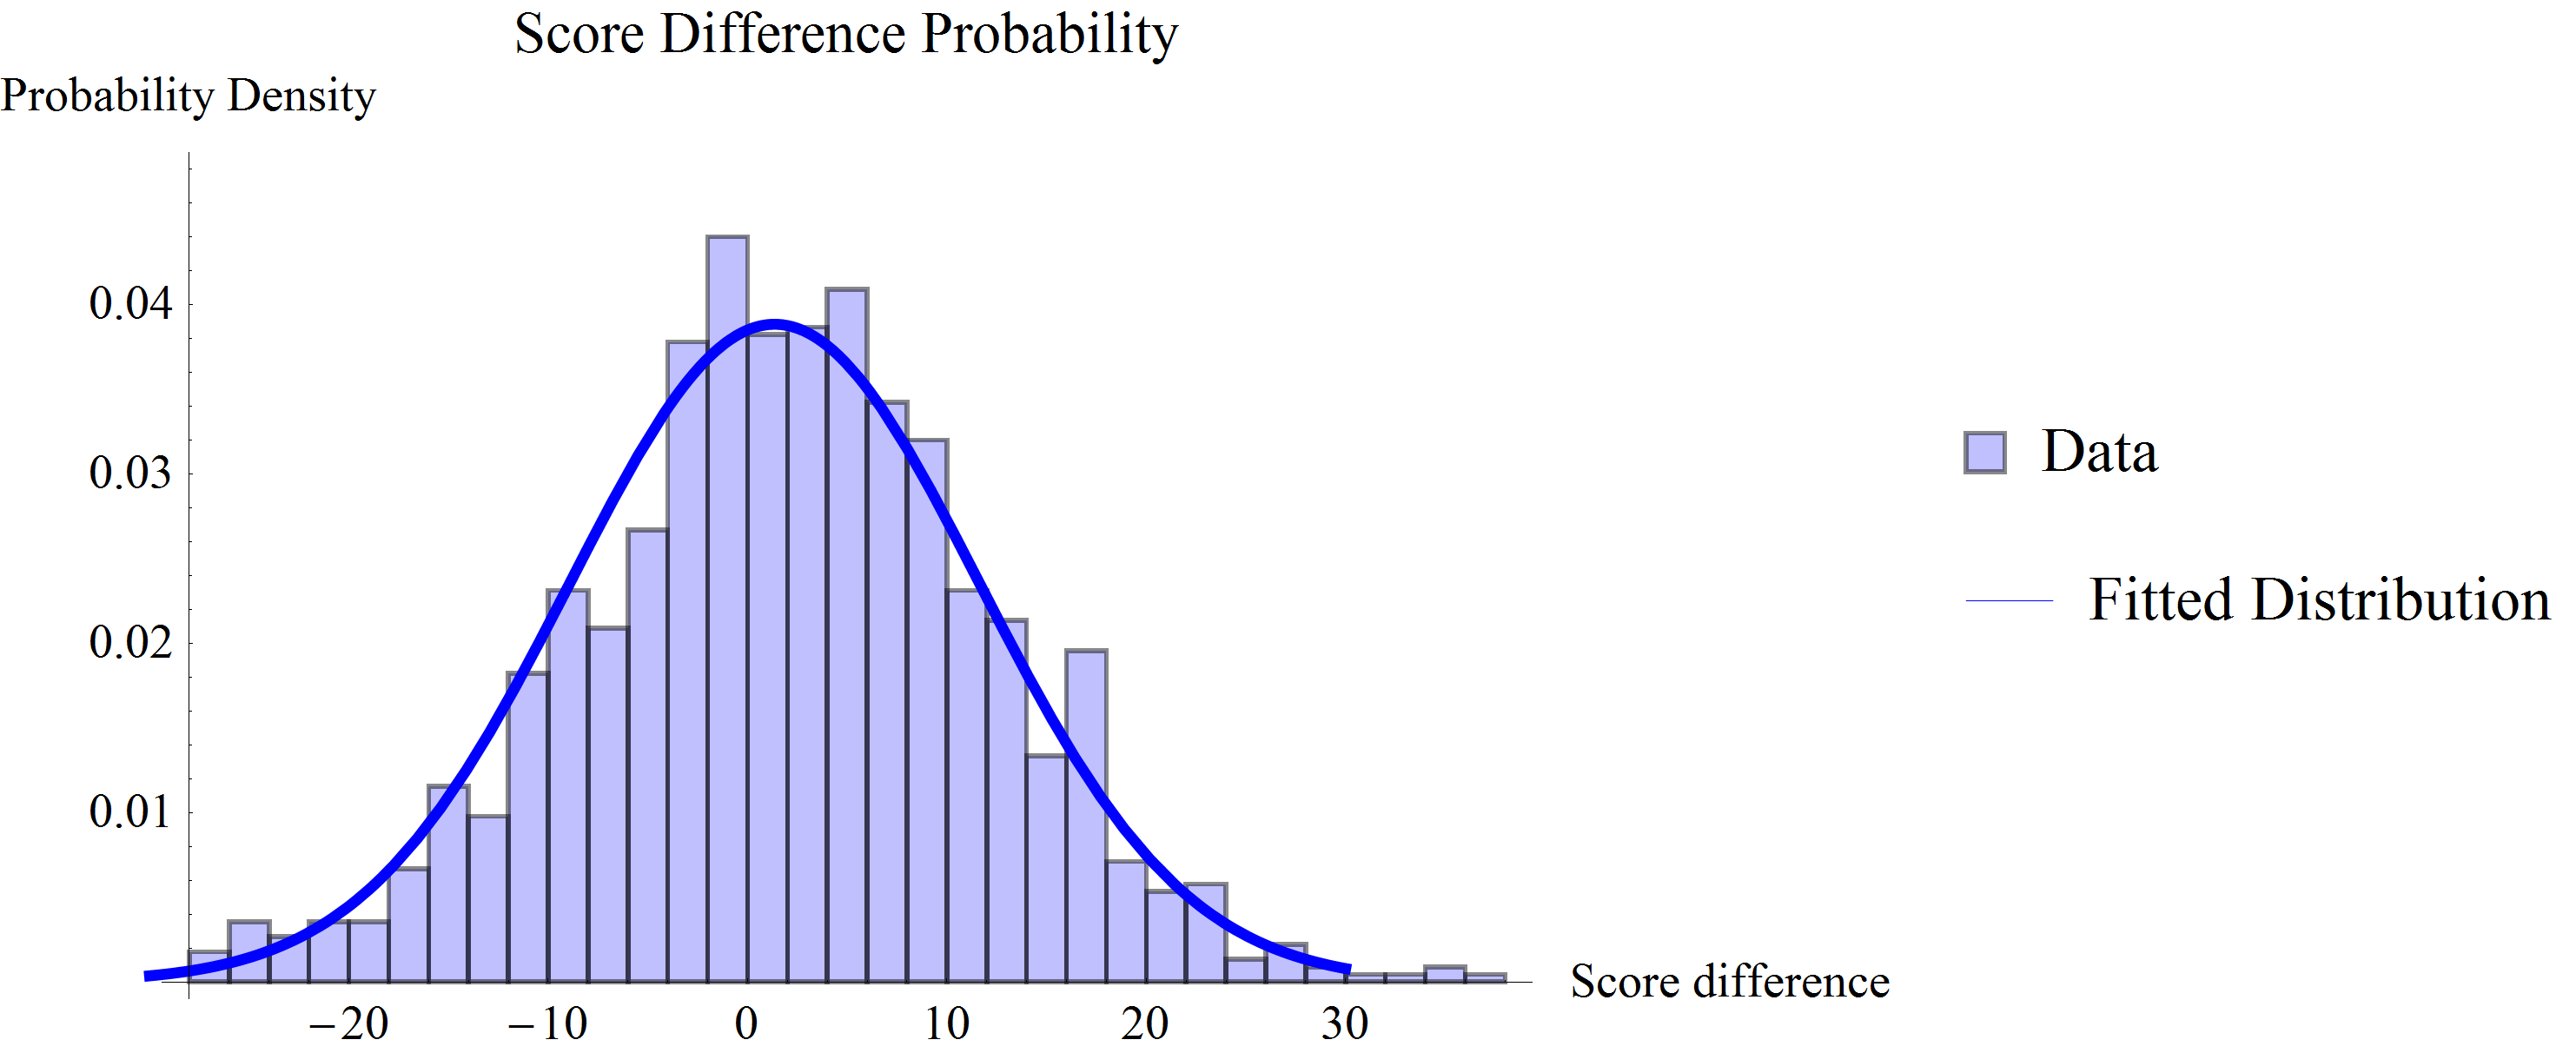
\includegraphics[scale=.6]{normalfit.png}
\caption{Example graphic indicating data and fitted normal distribution.}
\label{fig:normal}
\end{center}
\end{figure}

\subsection{In-Game Progression}
\label{sec:progression}
Now, let's characterize how the point difference changes throughout a game (on average). If we make the assumption that the play in each quarter is independent
(first quarter performance has no bearing on fourth quarter, etc.), then we should expect the general properties of adding independent Normally-distributed variables:
\begin{itemize}
\item{Taking $\mathcal{N}(\mu_1,\sigma_1)\pm\mathcal{N}(\mu_2,\sigma_2)$ gives a combined mean of $\mu=\mu_1\pm\mu_2$.}
\item{Taking $\mathcal{N}(\mu_1,\sigma_1)\pm\mathcal{N}(\mu_2,\sigma_2)$ gives a combined variance of $\sigma^2=\sigma_1^2+\sigma_2^2$ (variances \textit{always} add).}
\end{itemize}
Let's also assume (for the moment -- we'll test it momentarily) that each quarter is approximately the same ($\mu_1\approx\mu_2$, $\sigma_1\approx\sigma_2$, etc.).

From this, can you come up with a model for
the mean difference in score as a function of percentage of time played so far during a game? For the standard deviation of the difference in score as a function
of percentage of time played so far during a game? This creates functions $\mu(t)$ and $\sigma(t)$ where $t\in[0,1]$. We know the final score and spread from subsection~\ref{sec:results} ,
and we know the initial score and spread as well (starts at 0--0 with $\sigma=0$). In your report, please discuss how you arrived at the functions you did.

\textit{Hint:} $\mu(t)$ and $\sigma(t)$ should have the boundary properties outlined above: 
\begin{itemize}
\item{$\mu(0)=0$}
\item{$\sigma(0)=0$}
\item{$\mu(1)=\mu=\mu_1+\mu_2+\mu_3+\mu_4$}
\item{$\sigma^2(1)=\sigma^2=\sigma_1^2+\sigma_2^2+\sigma_3^2+\sigma_4^2$}
\end{itemize}
then also be able to predict the distribution at half-time ($\mu(.5)=\mu_1+\mu_2$, and $\sigma^2(.5)=\sigma_1^2+\sigma_2^2$). If this part stumps you, feel free to ask your student teachers about it.

\subsection{Model-Fitting Game Progression}
\label{sec:model}
With the model for $\mu(t),~\sigma(t)$ from subsection \ref{sec:progression}, use a \texttt{LinearModelFit} or \texttt{NonlinearModelFit} in \textit{Mathematica}
to fit the coefficient based on the data at each quarter (rather than just using the final distribution). For example, you'll have \textit{Mathematica} fit the function
$\mu(t)$ to the data:
$$\{\{0,~0\},~\{0.25,~\mu_1\},~\{0.5,~\mu_1+\mu_2\},~\{0.75,~\mu_1+\mu_2+\mu_3\},~\{1,~\mu_1+\mu_2+\mu_3+\mu_4\}\}$$
These fitting functions provide the estimate of the parameter \textit{and} the standard error in the parameter (use the 
``\texttt{ParameterTable}'' field of the fit -- see the documentation) along with the $p$-value. 

The $p$-value reported is the probability of getting an estimated
coefficient this far from $0$ if there is no dependence on the coefficient. For example, a $p$-value of $0.9$ says that $90\%$ of the time, we would fit a coefficient
this different from 0 where there really is no dependence. Based on the reported $p$-values, was the fit sufficient?

If so, using the estimate and error for the mean vs. time and for the standard deviation vs. time,
is the model based only on final scores consistent with the fitted data? More formally, are the coefficients used in the simple model from subsection \ref{sec:progression} consistent
with those determined by the fits in this subsection? How many ``standard errors'' away from each other are they? Is the difference statistically significant at the 
$99\%$ confidence level (i.e., should we be
surprised at the result from the simple model if it is indeed drawn from the one we fitted)?

\subsection{Results}
Using results from subsection \ref{sec:model}, present a visual indicating how all the games compare with the average and standard deviation of the distribution at the end of each quarter. You
may want to use the \texttt{ErrorListPlots} module in \textit{Mathematica}. Feel free to explore different representations and include them in your submitted \textit{Mathematica} document.

\subsection{Bonus: Single-Game Predictions}
Does the Home Field Advantage work for a specific team? Select a team and use a variation of the techniques above to determine if they are more likely to win home games or away games.

\subsection{Bonus: Working with Normal Distributions}
Using the same ``independence'' approximations above, find the actual score at half-time $D_2$ for a few games, then predict the probability the team should win, assuming the
game is representative. In other words, based on $\mu_{3-4}=\mu_3+\mu_4,~\sigma_{3-4}^2=\sigma_3^2+\sigma_4^2$ and $\mu_{f}=D_2+\mu_{3-4},~\sigma_f=\sigma_{3-4}$ (with
$D_2$ being the score difference at half-time), determine what certainty you have that the home team will win the game. 

\section{Hubble Constant}
Eureka! An undergraduate physicist at UT-Austin discovered a new type of supernova -- the Type XLIIeo! Fortunately, this
mystery physicist determined the peaks in the spectrum of Type XLIIeo supernovae and even took data from
distant examples! We may never know who this awesome person is, so there will be no Nobel prize awarded for the work.
Luckily for you, we've recovered the data that will let you investigate the evolution of the universe!

\subsection{The Model}
\label{sec:hmodel}
Type XLIIeo supernovae are characterized by the peak wavelengths and widths in Table \ref{tab:peaks}. Surprisingly, for
this type of supernovae, when signal is expressed as a function of wavelength, we get a scaled Gaussian distribution. The
light emitted is based on the relative output at each peak as follows:

\begin{equation}
\label{eq:spectrum}
S_{*}(\lambda)=\sum_i c_i\cdot \sigma_i \cdot\mathcal{N}[\lambda_i, \sigma_i](\lambda)
\end{equation}
where $c_i$ is the coefficient for the relative proportion of materials in the star (same for all Type XLIIeo stars),
$\lambda_i$ is each of the peak wavelengths (with $\sigma_i$ being the standard deviation in their distribution),
and $\mathcal{N}[\mu,\sigma](x)$ being the typically-defined Normal distribution as a function of $x$. This total distribution
and its component parts are visible in Figure \ref{fig:spectrum}.

\begin{table}
\begin{centering}
\begin{tabular}{|c|c|c|}
Peak $\lambda_i$ & $\sigma_i$ & $c_i$\\
\hline
\SI{1100}{\angstrom} & \SI{300}{\angstrom} & $1/12$\\
\SI{1250}{\angstrom} & \SI{8}{\angstrom}  & $1/6$\\
\SI{1400}{\angstrom} & \SI{50}{\angstrom} & $1/36$\\
\SI{1600}{\angstrom} & \SI{80}{\angstrom} & $1/4$\\
\SI{1750}{\angstrom} & \SI{20}{\angstrom} & $13/36$\\
\SI{1800}{\angstrom} & \SI{125}{\angstrom} & $1/9$
\end{tabular}
\caption{Peaks, widths, and relative abundance of each component in the signal. These may be visualized with Figure
\ref{fig:spectrum} and Equation \ref{eq:spectrum}.}
\label{tab:peaks}
\end{centering}
\end{table}

\begin{figure}
\begin{center}
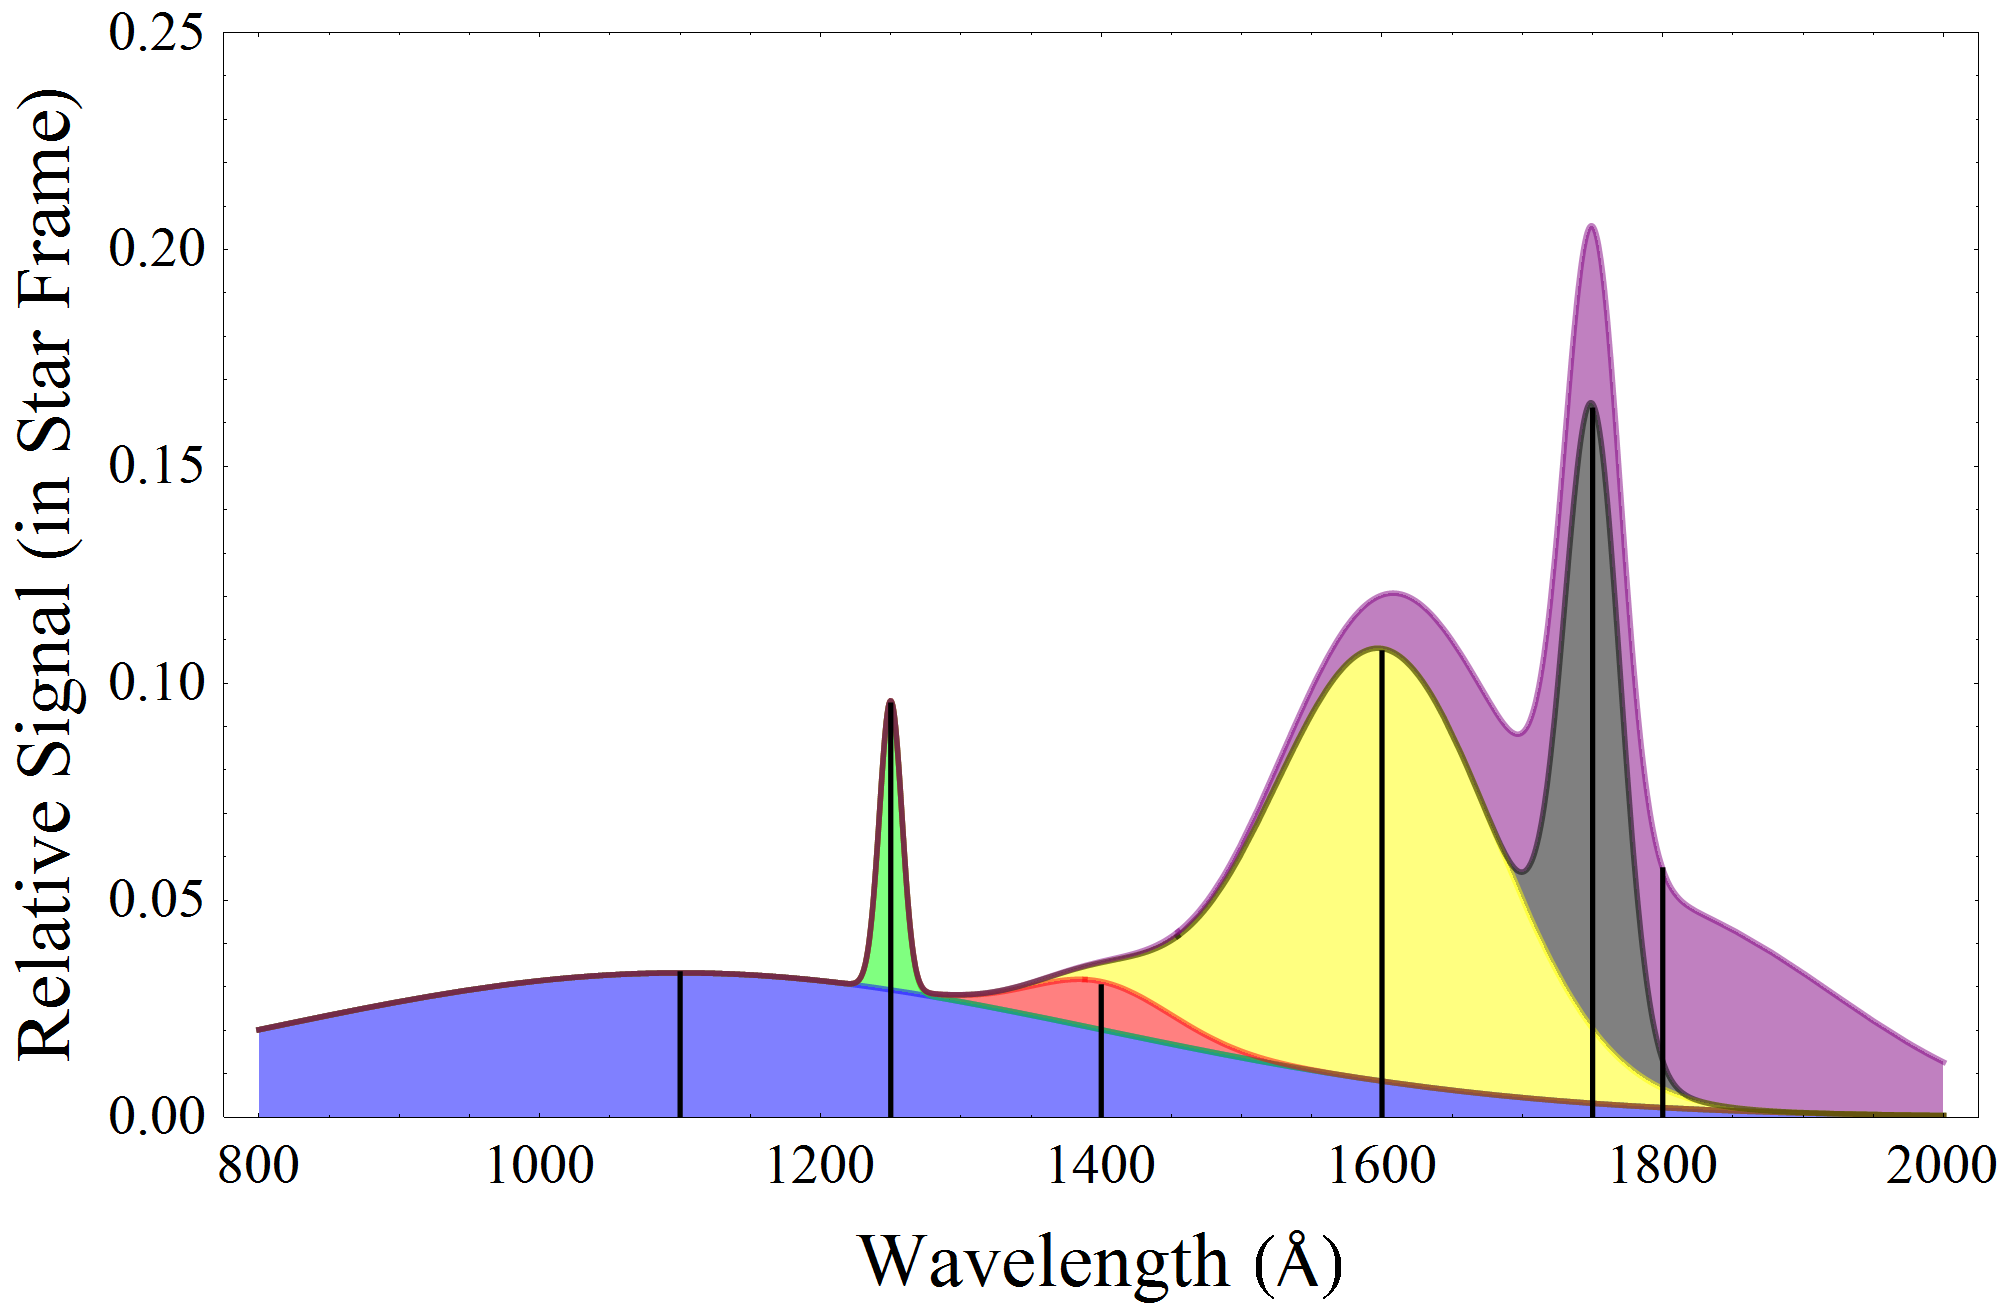
\includegraphics[scale=.95]{hubblecontrib.png}
\caption{Contribution to signal from each peak wavelength. Largest point on distribution is total signal emitted
in the reference frame of the star. Peak of each component distribution is marked with a black line.}
\label{fig:spectrum}
\end{center}
\end{figure}

Now that we have a model for a Type XLIIeo supernova's output, we now have to consider two important factors.
First, the Doppler effect. This states that the observed wavelength on Earth $\lambda_{E}$ will be shifted
from the original wavelength $\lambda_0$ based on the velocity of the star toward Earth:

\begin{equation}
\lambda_E=\sqrt{\frac{c+v}{c-v}}\lambda_0
\end{equation}
with $v>0$ being the star moving away, and $c$ being the speed of light (this is the relativistic version). So each
peak (in fact, each point in the data) should be shifted by $\lambda_0\rightarrow\sqrt{\frac{c+v}{c-v}}\lambda_0$.
We also have to modify our standard deviation by the same factor (to convince yourself of this, consider shifting
the mean $\lambda_i$ and a point one standard deviation away $\lambda_i+\sigma_i$).

Secondly, we must consider the effect of distance on the signal we get. If we assume each Type XLIIeo supernova is identical
in terms of output, then the signal should be proportional to $1/d^2$, where $d$ is the distance to the star from Earth.

\subsection{Analysis}
\label{sec:hanalysis}
Given the model in subsection \ref{sec:hmodel}, and the data \href{http://www.cs.utexas.edu/~evanott/PHY110C_Textbook/static/data_analysis/_downloads/hubble.csv}{here},
you will determine the Hubble constant. The Hubble Law says that the velocity of a galaxy away from Earth is related
to the distance by $$v=H_0d$$ This says that things that are farther away move away faster.\footnote{This expansion is 
caused by dark energy, and is consistent with a ``metric expansion'' of space. If we center our coordinate system at
any given point, it will look like all space is expanding away from it. Cosmologists consider the universe to be
isotropic (same in every direction) and to obey the Copernican principle (no preferred center).}

The data are already in a convenient form. After using \texttt{Import}, the first dimension has the data for 15
different stars. Each star's data is a list of points $(\lambda,~S(\lambda))$. Use this data, and the fact that the first
set of data is \SI{3}{Mpc} away (for scaling) to determine what the distance and velocity of each star is. From this,
use the Hubble Law to obtain the Hubble constant. \textit{Hint:} You will likely want to use the \texttt{NonlinearModelFit} function
with $1000$ maximum iterations and the ``NMaximize'' method of calculation.

What bounds can you place on the Hubble constant based on this data from error in estimating parameters from the model fit? 
What about the distribution of values you get for $H_0$ from each star? Which contributes most to the width of your estimate? Please
report the Hubble constant in the ``traditional'' units of \si{(\kilo\m\per\s)\per Mpc}.

\section{Modern Lab}
\label{sec:modern}
For those of you already in PHY 353L, this option is intended to allow you to refine a past lab report to show us
your mastery of \textit{Mathematica} and \LaTeX. If you choose this option, you will need to also produce a dataset
(preferably a CSV file or other portable document type) in addition to your \textit{Mathematica} and \LaTeX~files.

\subsection{Data Requirements}
Reduce your original data to only the required information and provide it in an easy-to-import file. For example,
the Hubble Law option above simply gives wavelength and signal, as those are the only relevant parameters, not the
output of an extraneous oscilloscope, not the time the data were collected (unless that is important), etc. Furthermore,
this file should have headers that are strings (like the basketball data) that describe the data.

\subsection{\textit{Mathematica} Requirements}
Provide a simple \textit{Mathematica} document that flows from data input to final calculations and graphs. We should
be able to execute the code in the order it appears on the page to produce results. Furthermore, each line should be
relevant to the final results. We have no idea which project you'll choose to write about, so you will need to write
very clear code with significant comments for us to see what your code is doing. You should also make very
clear graphs, ideally with histograms, best-fit lines, theoretical behavior, etc.

\subsection{\LaTeX Requirements}
This is not Modern Lab. In this class, we are less interested in the specifics of your experimental setup or historical context.
Your write-up should be done in \LaTeX, detailing how the data are represented (see the example in Table \ref{tab:data}),
the math you used to transform your raw data into results, how you put bounds on your final result(s), the plots, etc.
Your writing need not be overly technical or primed for publication. You are free to talk about the actual code as well
if you did something you found interesting or helpful. We'll use your \LaTeX~code for two purposes: to read
about your methods of data analysis, and to see your mastery of the \LaTeX~language. We should see advanced packages,
formatting, etc.

\begin{thebibliography}{9}
\bibitem{basketballgeek} \url{http://www.basketballgeek.com/downloads/2008-2009.regular_season.zip}
\end{thebibliography}

\end{document}